\documentclass[main.tex]{subfiles}
\begin{document}
在\S\ref{I.2 pratical_thermodynamics}中已经提到,要确定混合物系统的完整热力学性质,除了需要知道它的某一可逆过程热容关于系统状态的完整函数外,还需要知道其$pVTn_i$状态方程。这样,就能依照偏摩尔量的测量原理,把确定各组份化学势所需的偏摩尔响应函数都获知,以便确定系统最基本的热力学函数——内能和熵——的微分表达式。

但是,这样的实验工作量会随组份数的增多而成倍增加。我们朴素地问,能否仅测量各组份\emph{纯物质}的性质$M_i^*\left(X,Y\right)$,就能通过形如
\[M\left(X,Y,\left\{n_i\right\}\right)=\sum_i n_i M_i^*\left(X,Y\right)\]
的加和性,得到混合物同样条件下任一组成$\left\{n_i\right\}$的性质$M\left(X,Y,\left\{n_i\right\}\right)$了呢?——很遗憾,这种针对纯物质性质的加和性并不普遍成立。对所有系统普适的加和性只有偏摩尔量的加和性(式\eqref{eq:II.2_additivity_partial_molar_quantity_1}或\eqref{eq:II.2_additivity_partial_molar_quantity_2})。可是,回忆《物理化学》的知识,道尔顿分压定律好像就是形如上式的某种针对纯物质的加和性呀。再联想到,道尔顿分压定律是仅适用于理想气体的混合物的。那么,至少如果我们仅讨论理想气体的混合物,是否就能够利用道尔顿分压定律,来证明系统其他各热力学性质也均满足上面这种针对其纯物质性质的加和性呢?答案仍是否定的。本节将讨论这个问题,并最终确定理想的气体混合物的完整定义。

我们知道\footnote{见《物理化学》\S1.1之“气体分子运动公式对几个经验定律的说明”。},理想气体除了在单组份的情况下满足
\begin{enumerate}
  \item 玻意耳定律:$pV=\text{温度的函数}$;
  \item 焦耳定律:内能是温度的函数\footnote{亦可见《物理化学》\S 2.8式(2.18)。};
  \item 阿伏伽德罗定律:同温同压下,一摩尔各种气体的体积相等;
\end{enumerate}
这三条之外,在多组份的情况下还要满足道尔顿分压定律。而后者说的就是多组份气体混合物压强的这样一种加和性:\emph{混合气体的压强等于各组份气体同温同体积下的压强之和},写成式子就是
\[p\left(T,V,\left\{n_i\right\}\right)=\sum_i p^*_i\left(T,V\right)\]
其中$p_i^*\left(T,V\right)$是组份$i$纯物质的压强。也许很多读者未必立刻完全理解这个式子的含义。它的意思是说,我们如果打算以组成$\left\{n_i\right\}$来混合各组份的纯物质,想知道混合后的气体在温度为$T$和体积为$V$下的压强$p$,一方面我们可以直接测出来,得到上式等号左边;另一方面我们可以尝试把各组份纯物质置于温度同样为$T$、体积同样为$V$的容器中,测量它们各自的压强$p_i^*$,然后把这些压强加起来,得到上式等号右边。它们当然不一定相等。如果它们不仅在这一次实验中相等,而且对无论什么温度$T$、体积$V$和组成$\left\{n_i\right\}$都相等,那么我们就说这个气体混合物满足道尔顿分压定律。仅在这个表述中,我们没有要求这些气体在混合前都是理想气体;它们可以不是理想气体,却满足这种混合加和性。如果这些组份的纯物质在相同的条件下也都是理想气体,则有$p_i^*\left(T,V\right)=n_iRT/V$,由道尔顿分压定律可得$p=\sum_in_iRT/V=nRT/V$,即混合后的系统将仍是一个理想气体——这是各纯份纯物质气体皆为理想气体同时它们的混合物满足道尔顿分压定律时的特殊结论。但凡其中一个组份纯物质不是理想气体,都没有这个结论。可见,道尔顿分压定律是独立于前三条(即理想气体)定律的;满足道尔顿分压定律的混合物未必是理想气体的混合物。

这四条定律,似乎给出了一个气体混合物的$pVTn_i$状态方程,即$V\left(T,p,\left\{n_i\right\}\right)=RT\sum_in_i/p$。尽管还缺少热容,但至少应该足以预测系统在任一等温实验下的性质了。以下这个实例说明,仅从上列四条定律,也不足以预测气体混合物在等温实验的热力学行为。

考虑如图\ref{fig:gas_mixture_experiment}所示的实验。整个系统与环境保持温度为$T$。达到平衡时,左侧硬壁缸内的混合气体压强为$p$,右侧为一系列品质相同的气球,经过半透膜的分隔,它们各只含有纯气体$i$,气球膨胀的大小可反映气球内的压强大小$p^*_i$(示意图中显得一样大了)。

$p^*_i$各是多少一般将取决于左侧混合气体的组成$\left\{x_i\right\}$ 。但是仅靠道尔顿分压定律和基本热力学关系,是无法给出右侧各气球的压强$p^*_i$具体应是多少的——哪怕我们再假定所有腔室中的气体是理想气体。也就是说,右腔室的气体行为如何依赖左侧混合气体的性质,可以随具体系统的化学差异而不同。我们于是规定,作为模型系统的\emph{理想的气体混合物(ideal gas mixture)},不仅每个组份纯物质是理想气体,而且在这样的实验中,给定温度$T$的平衡态下,任一能通过半透膜的组份$i$,在膜右边的纯物质腔室中的压强满足:
\begin{equation}
  \label{eq:II.3_ideal_gas_mixture_partial_pressure_rule}
  p^*_i\left(T\right)=x_ip\left(T\right),\quad\text{理想的气体混合物}
\end{equation}
可见,我们对理想的气体混合物直接规定了在这个问题当中右边腔室压强与左侧腔室性质的定量关系。

值得提醒的是,此处的$p$和$p_i^*$跟前面道尔顿分压定律表达式中的$p$和$p_i^*$情况不一样。在道尔顿分压定律的表达式中,$p$和$p_i^*$是同温同体积的,但在这个问题当中各右腔室的体积一般不等于左腔体积,所以在这个问题中不能根据道尔顿分压定律说$p=\sum_ip_i^*$。

\begin{figure}[ht]
  \centering
  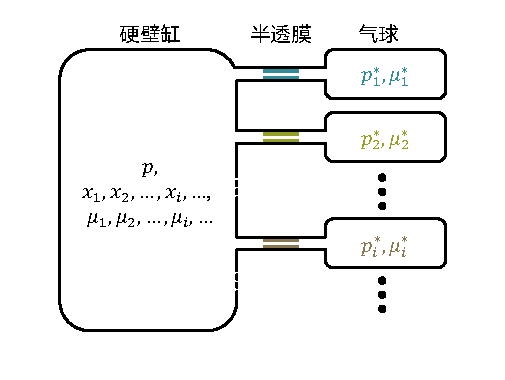
\includegraphics{../images/gas_mixture_experiment.pdf}
  \caption{确定气体混合物行为的实验示意图。整个系统与环境保持温度为$T$。达到平衡时左侧硬壁缸内的混合气体压强为$p$,右侧为一系列同品质的气球,经半透膜,它们只含有纯气体$i$,气球膨胀的大小可反映气球内的压强大小$p^*_i$(示意图中显得一样大了)。$p^*_i$各是多少一般将取决于左侧混合气体的组成$x_1,x_2,\cdots,x_i,\cdots$,但具体取决方式依赖气体混合物的状态方程。理想的气体混合物满足$p^*_i=x_ip$。}
  \label{fig:gas_mixture_experiment}
\end{figure}

有了式\eqref{eq:II.3_ideal_gas_mixture_partial_pressure_rule},我们确实可以推导这个问题的完整热力学信息。由于膜右室是单组份理想气体,由$\mu_i^*=\mu_i^*\left(T,p\right)$的全微分,加上恒温过程$\mathrm{d}T=0$的条件,可以得到
\begin{align*}
  \mathrm{d}\mu_i^* & =\left.\frac{\partial\mu_i^*}{\partial p}\right|_{T}\mathrm{d}p \\
                    & =V_i^*\left(T,p\right)\mathrm{d}p                               \\
                    & =\frac{RT}{p}\mathrm{d}p=RT\mathrm{d}\ln p
\end{align*}
因此由相平衡条件$\mu_i=\mu_i^*$和理想的气体混合物的规定(式\eqref{eq:II.3_ideal_gas_mixture_partial_pressure_rule}),
\[\mathrm{d}\mu_i=\mathrm{d}\mu_i^*=RT\mathrm{d}\ln p_i^*=RT\mathrm{d}\ln\left(x_ip\right)\]
以上要对所有组份$i$均成立。可见,系统这一特定实验中的性质规定,其实是规定了理想的气体混合物的偏摩尔吉布斯自由能的表达形式。因此,我们为理想的气体混合物写下如下定义性质的化学势表达式:恒定$T$下,理想的气体混合物的任意组份$i$的化学势均满足
\begin{equation}\label{eq:II.3_def_ideal_gas_mixture_mu}
  \mathrm{d}\mu_i^\text{ig}\left(T,p,\left\{n_j\right\}\right)=RT\mathrm{d}\ln\left(x_i p\right)
\end{equation}
其中上标“ig”表示理想的气体混合物,注意,得到这个化学势形式的推导过程中,我们用到了“每个组份纯物质气体是理想气体”的条件,所以这个等式等价于每个组份满足所有三条理想气体经验定律,再加上关于混合行为的式\eqref{eq:II.3_ideal_gas_mixture_partial_pressure_rule}的条件。这跟理想的气体混合物的文字定义一致,因此也可以直接用上式定义理想的气体混合物。

我们分析一下这个式子蕴含的意义。作为一个状态函数,组份$i$在理想的气体混合物中的化学势$\mu_i^\text{ig}$自然应是状态参量$\left(T,p,\left\{n_i\right\}\right)$的函数。它在恒定$T$($\mathrm{d}T=0$)下的微分式理应形如
\[\mathrm{d}\mu_i^\text{ig}\left(T,p,\left\{n_j\right\}\right)=\left.\frac{\partial \mu_i^\text{ig}}{\partial p}\right|_{T,\left\{n_j\right\}}\mathrm{d}p+\sum_j\left.\frac{\partial\mu_i^\text{ig}}{\partial n_j}\right|_{T,p,\left\{n_{k\neq j}\right\}}\mathrm{d}n_j\]
而式\eqref{eq:II.3_def_ideal_gas_mixture_mu}等号右边的微分式$\mathrm{d}\ln\left(x_ip\right)$可推算至以下形式
\[\mathrm{d}\ln\left(x_ip\right)=\mathrm{d}\ln p+\mathrm{d}\ln n_i\]
其中用到了$x_i=n_i/\sum_jn_j$以及系统总摩尔数恒定(封闭系统)$\mathrm{d}n=\sum_i\mathrm{d}n_i=0$。故有
\begin{align*}
  \left.\frac{\partial \mu_i^\text{ig}}{\partial p}\right|_{T,\left\{n_j\right\}}             & =V_i^\text{ig}=RT\mathrm{d}\ln p                                                \\
  \left.\frac{\partial \mu_i^\text{ig}}{\partial n_j}\right|_{T,p,\left\{n_{k\neq j}\right\}} & =\left\{\begin{array}{ll}0,&j\neq i\\RT\mathrm{d}\ln n_i,&j=i\end{array}\right.
\end{align*}

理想的气体混合物化学势定义式\eqref{eq:II.3_def_ideal_gas_mixture_mu}是以微分关系的形式给出的。我们之所以不直接用明显的表达式来定义这个模型系统,是因为热力学函数的绝对值是不易知的,只有其变化量是易于讨论的。用微分表达式来规定规律性,可供我们随时通过式\eqref{eq:I.1_integral_of_function}来进行任意状态之间的热力学函数变化量,有最好的一般性和灵活性。所以我们要习惯用微分关系来定义模型系统的方式。例如,我们可任选某压强值$p^\circ$作为参考压强,则理想的气体混合物等温等组分的体积变化过程各组份的化学势变化就是
\begin{equation}\label{eq:II.3_ideal_gas_mixture_mu_p0}
  \begin{aligned}
    \mu_i^\text{ig}\left(T,p,\left\{n_j\right\}\right)-\mu_i^\text{ig}\left(T,p^\circ,\left\{n_j\right\}\right) & =\int_{p^\circ}^p\mathrm{d}\mu_i^\text{ig}\left(T,p^\prime,\left\{n_j\right\}\right) \\
                                                                                                                & =RT\int_{p^\circ}^p\mathrm{d}\ln\left(x_ip^\prime\right)                             \\
                                                                                                                & =RT\ln\left(\frac{x_ip}{p^\circ}\right)
  \end{aligned}
\end{equation}
《物理化学》书上的理想的气体混合物化学势的定义式(\S 4.5式(4.31))只是具体选择$p^\circ=p\stst$作为惯例而已。

总结理想的气体混合物一共要遵守的定律就是:气体混合物在任何组成下遵循式\eqref{eq:II.3_def_ideal_gas_mixture_mu}或等价地——
\begin{enumerate}
  \item 玻意耳定律:$pV=\text{温度的函数}$;
  \item 焦耳定律:内能是温度的函数\footnote{亦可见《物理化学》\S 2.8式(2.18)。};
  \item 阿伏伽德罗定律:同温同压下,一摩尔各种气体的体积相等;
  \item 道尔顿分压定律加强版:给定温度$T$的平衡态下,任一能通过半透膜的组份$i$,在膜两边的分压相等。
\end{enumerate}

式\eqref{eq:II.3_def_ideal_gas_mixture_mu}足以给出理想的气体混合物的完整热力学性质,以下列出部分。由式\eqref{eq:I.1_Maxwell_GnT}和式\eqref{eq:I.1_Maxwell_GTp}有,
\begin{align}
  S^\text{ig}_i & =-\left.\frac{\partial \mu^\text{ig}_i\left(T,p,\left\{n_j\right\}\right)}{\partial T}\right|_{p,\left\{n_j\right\}}=S_i^{\circ,\text{ig}}-R\left[\ln x_i+\ln \left(p/p^\circ\right)\right] \\
  V^\text{ig}_i & =\left.\frac{\partial\mu^\text{ig}_i\left(T,p,\left\{n_j\right\}\right)}{\partial p}\right|_{T,\left\{n_j\right\}}=\frac{RT}{p}
\end{align}
其中$S_i^{\circ,\text{ig}}\equiv-\left(\partial\mu_i^\text{ig}\left(T,p^\circ,\left\{n_j\right\}\right)/\partial T\right)_{\left\{n_i\right\}}$。恒压恒组成下,又由式\eqref{eq:I.1_heat_capacity_entropy_p}和式\eqref{eq:I.1_Maxwell_GTp}有
\begin{align}
  \left.\frac{\partial S^\text{ig}}{\partial T}\right|_{p,\left\{n_i\right\}} & =\frac{C_p}{T} \\
  \left.\frac{\partial S^\text{ig}}{\partial p}\right|_{T,\left\{n_i\right\}} & =-\frac{nR}{p}
\end{align}
故理想的气体混合物的熵的完整全微分式是
\[\mathrm{d}S^\text{ig}=\frac{C_p}{T}\mathrm{d}T-\frac{nR}{p}\mathrm{d}p+\sum_i\left[S_i^{\circ,\text{ig}}-R\ln x_i-R\ln\left(p/p^\circ\right)\right]\mathrm{d}n_i\]
恒定$T$、$p$下,由偏摩尔量加和性,
\[S^\text{ig}\left(T,p,\left\{n_i\right\}\right)=\sum_in_i\left[S_i^{\circ,\text{ig}}-R\ln x_i-R\ln\left(p/ p^\circ\right)\right]\]
故同条件下的混合熵变(即把$n_1,n_2,\cdots$纯物质混合为组成是$\left\{n_i\right\}$的气体混合物的熵变)
\begin{align*}
  \Delta_\text{mix}S^\text{ig} & =S^\text{ig}\left(T,p,\left\{n_i\right\}\right)-\sum_i n_i S^\text{*,ig}\left(T,p\right)                                                                \\
                               & =\sum_in_i\left[S_i^{\circ,\text{ig}}-R\ln x_i-R\ln\left(p/p^\circ\right)\right]-\sum_in_i\left[S_i^{\circ,\text{ig}}-R\ln\left(p/p^\circ\right)\right] \\
                               & =-R\sum_in_i\ln x_i
\end{align*}
其中利用到纯物质$S_i^{*,\text{ig}}=S_i^\text{ig}\left(T,p,x_i=1\right)$。

然后我们推导一下混合吉布斯自由能变。利用偏摩尔量的加和性,
\begin{align*}
  \Delta_\text{mix}G^\text{ig} & =G^\text{ig}\left(T,p,\left\{n_i\right\}\right)-G^\text{*,ig}\left(T,p\right)                               \\
                               & =\sum_in_i\left(\mu_i^\text{ig}\left(T,p,\left\{n_j\right\}\right)-\mu_i^\text{*,ig}\left(T,p\right)\right)
\end{align*}
而由式\eqref{eq:II.3_def_ideal_gas_mixture_mu},
\[\mu_i^\text{ig}\left(T,p,\left\{n_j\right\}\right)-\mu_i^\text{*,ig}\left(T,p\right)=RT\int_{1}^{x_i}d\ln\left(x_i^\prime p\right)=RT\ln x_i\]
故有
\[\Delta_\text{mix}G^\text{ig}=RT\sum_in_i\ln x_i=-T\Delta_\text{mix}S^\text{ig}\Rightarrow\Delta_\text{mix}H^\text{ig}=0\]
其中后面的等号和结论是与混合熵变的表达式比较而得。这些都是理想的气体混合物的重要的热力学特征。带$\Delta_\text{mix}$的函数变化量叫混合函数,这将在\S\ref{sec:II.4 real_mixture}节详细讨论。在这里我们仅需说明,按混合函数的定义,若任一系统的某一性质的混合函数为零,就说明该性质具有针对其各组份纯物质性质的加和性——这是对本节开头提出的问题的回应。
\end{document}